\documentclass[11pt]{article}
\usepackage{amssymb}
\usepackage{amsmath}
\usepackage{amsthm}
%\usepackage{fullpage}
\usepackage{comment}
\usepackage{hyperref}
\usepackage{graphicx}
\usepackage{clrscode3e}
\usepackage[font=scriptsize]{caption}
\usepackage{fancyhdr}
\usepackage[margin=1in]{geometry}
\usepackage{enumitem}
\usepackage{tikz}
\usepackage{enumitem}
\usetikzlibrary{shapes}

\includecomment{solution}
\includecomment{question}
\setlength{\parskip}{1ex}
\def\nats {{\mathbb N}}
\def\ints {{\mathbb Z}}
\def\R {{\mathbb R}}
\DeclareMathOperator*{\Argmin}{argmin}
\DeclareMathOperator*{\Argmax}{argmax}
\newcommand{\Implies}{\mbox{ IMPLIES }}
\newcommand{\Or}{\mbox{ OR }}
\renewcommand{\And}{\mbox{ AND }}
\newcommand{\Not}{\mbox{NOT }}
\newcommand{\Iff}{\mbox{ IFF }}
\newcommand{\True}{\mbox{True}}
\newcommand{\False}{\mbox{False}}

\newcommand{\Exp}{\mathbb{E}}
\newcommand{\Var}{\mathrm{Var}}

\newcommand{\cvec}[2]{\big[\begin{smallmatrix} #1 \\ #2 \end{smallmatrix}\big]}
\newcommand{\Cvec}[2]{\begin{bmatrix} #1 \\ #2 \end{bmatrix}}

\newcommand*{\Scale}[2][4]{\scalebox{#1}{$#2$}}
\newcommand*{\Resize}[2]{\resizebox{#1}{!}{$#2$}}

\newtheorem{theorem}{Theorem}
\newtheorem{lemma}{Lemma}
\newtheorem{corollary}[lemma]{Corollary}

\pagestyle{fancy}
\fancyhf{}
\rhead{Assignment 1}
\chead{Kevin Gao (1006967338)}
\lhead{CSC 2420}
\cfoot{\thepage}

\begin{document}

\section*{Assignment 1}

\begin{enumerate}[leftmargin=16pt]
    \item \textbf{Makespan}
    \begin{enumerate}[leftmargin=16pt]
        \item Argue for $m=2$ (resp. $m=3$) machines that any (not necessarily greedy) deterministic online algorithm would have competitive ratio no better than $\frac{3}{2}$ (resp. $\frac{5}{3}$) so that the natural greedy online algorithm approximation is tight for $m = 2$ and $m = 3$ for any online algorithm.
        \begin{proof}
            For $m = 2$, consider the following adversary strategy. Let $ALG$ be any deterministic online algorithm.
            \begin{itemize}
                \item If $ALG$ schedules the first two jobs on the same machine, then the adversary can stop after giving $(1,1)$ as the input. $ALG = 2$ whereas $OPT = 1$ since the optimal solution would scheduling the two jobs on two separate machines.
                \item If $ALG$ schedules the first two jobs on separate machines, the adversary can give $(1,1,2)$ as the input. $ALG = 3$ whereas $OPT = 2$. 
            \end{itemize}
            In both cases, $\frac{ALG}{OPT} \geq \frac{3}{2}$.

            For $m = 3$. The adversarial input is $(1,1,1,3,3,3,6)$.
            \begin{itemize}
                \item If $ALG$ does not schedule the first 3 jobs on 3 different machines, the adversary stops after giving $(1,1,1)$, resulting in a makespan of 3, but $C_{OPT} = 1$, so $\frac{ALG}{OPT} = 3$.
                \item If $ALG$ schedules the first 3 jobs on 3 different machines but does not schedule the second 3 jobs on 3 different machines, the adversary stops after giving $(1,1,1,3,3,3)$ and the makespan is at least 7 since one machine must have received at least two jobs of weight 3. But $OPT = 4$ which can be achieved by scheduling the first 3 jobs and the second 3 jobs evenly across 3 machines. Hence, $\frac{ALG}{OPT} = \frac{7}{4}$.
                \item Otherwise, the adversary gives $(1,1,1,3,3,3,6)$, which forces a makespan of 10 whereas $OPT = 6$ which can be achieved by putting the job of weight 6 on a separate machine and distribute the remaining jobs evenly across the remaining 2 machines. $\frac{ALG}{OPT} = \frac{10}{6} = \frac{5}{3}$.
            \end{itemize}
            In all cases, $\frac{ALG}{OPT} \geq \frac{5}{3}$. The adversary strategy for the 3-machine case can be illustrated by the decision tree shown below.
            \begin{figure}[htbp]
                \centering
                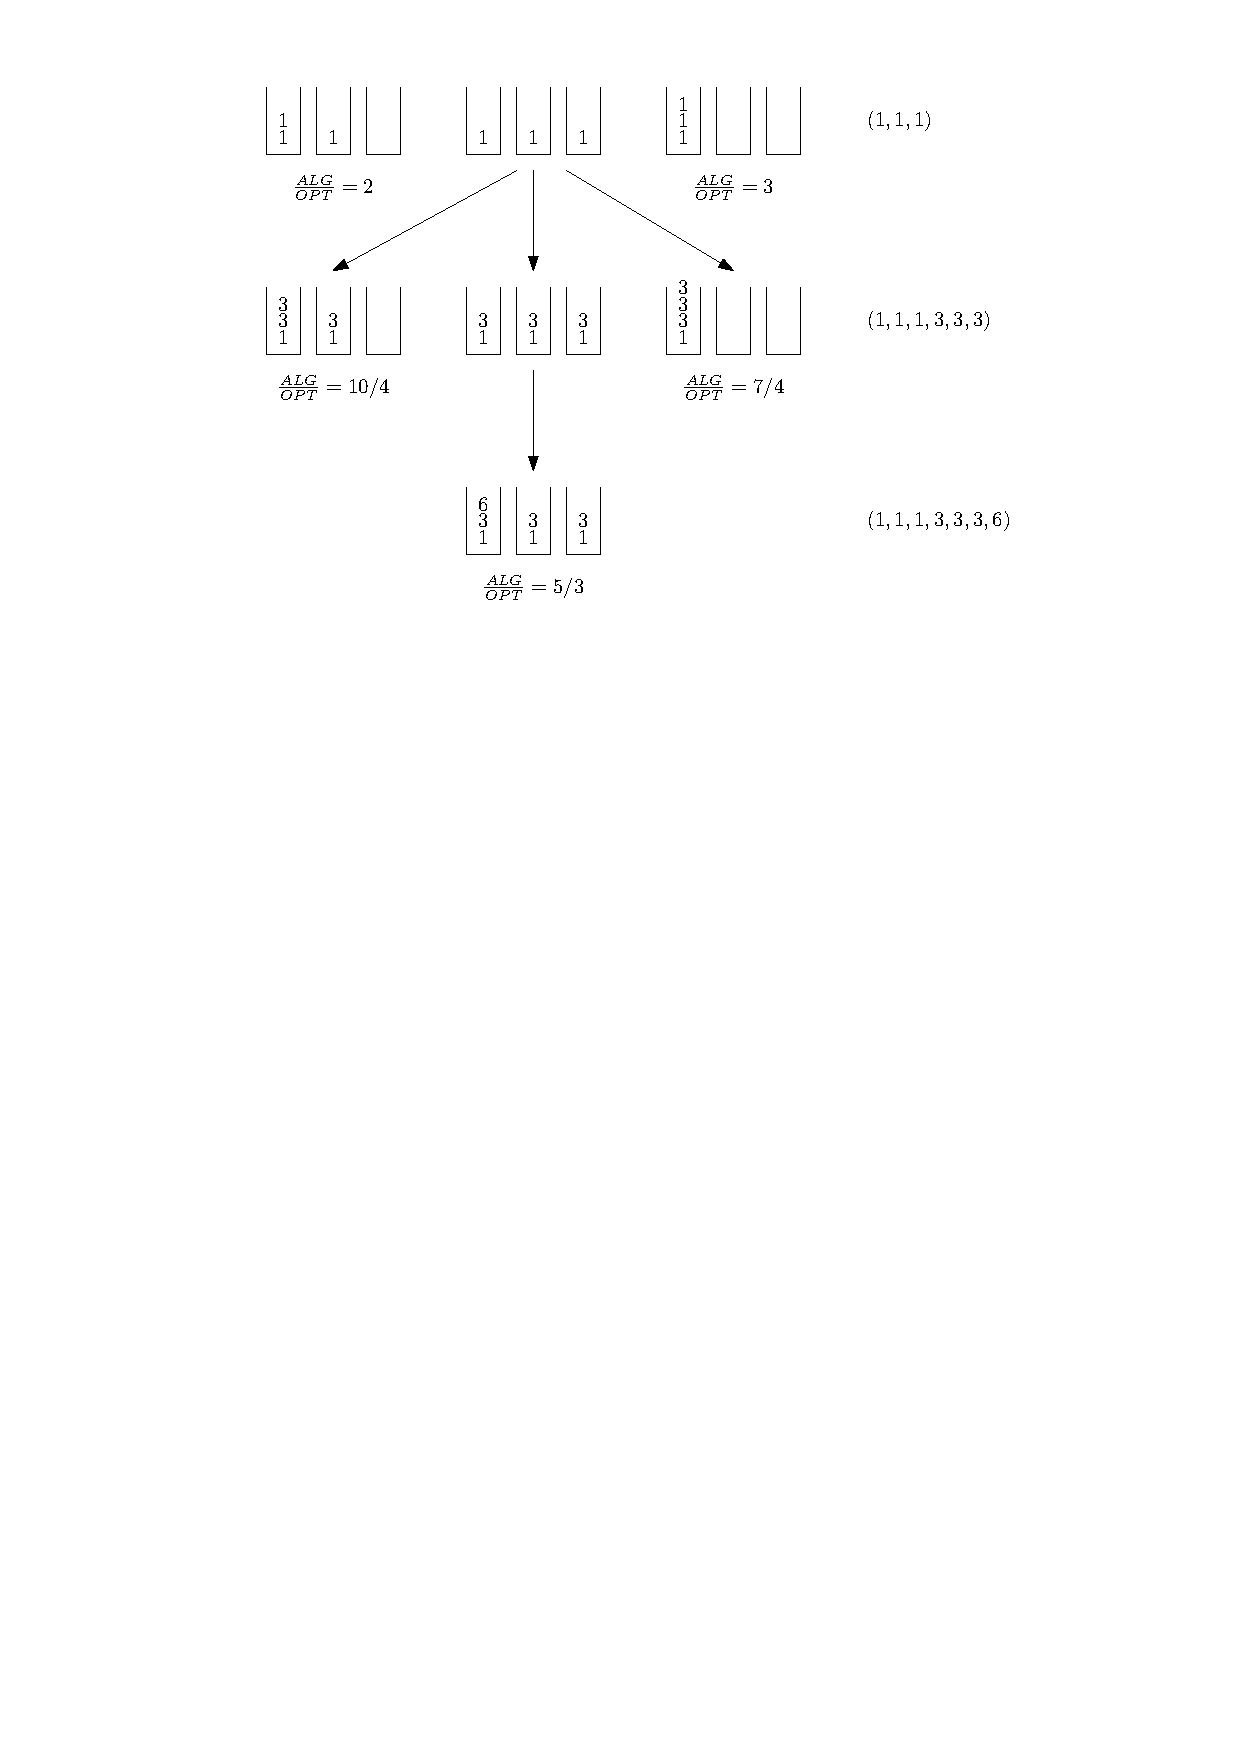
\includegraphics[width=0.6\linewidth]{figures/makespan-adv.pdf}
                \caption{Adversarial strategy for 3 machine.}
                \label{fig:makespan-adv}
            \end{figure}
        \end{proof}

        \item Consider the nemesis sequence (i.e. $p_i = 1$ for $1 \leq i \leq m(m - 1)$ and $p_{m(m-1)+1} = m$) that forces the ratio $2-1/m$ for Graham's greedy algorithm. Consider the same sequence for the makespan problem on m machines but now in the random order model (ROM). Provide a ``good" estimate for the expected competitive ratio of Graham's greedy algorithm iwhen executed on this set of inputs? Note: the expectation is wrt to the randomness in choosing the sequence uniformly at random.
        
        \begin{proof}
            Consider the partition of the $m(m-1)+1$ jobs into $m$ blocks. The first $m-1$ block will each contain $m$ jobs of size 1 and the last block will contain 1 job of size $m$. We will call the jobs of size 1 small jobs and the jobs of size $m$ large jobs. Observe that the resulting makespan from running Graham's algorithm is equal to the size of the largest job plus the load on the least loaded machine when the last large job is scheduled. As soon as one large job is scheduled, the machine will no longer accept any more jobs.

            If the large job arrives when there are between 0 and $m-1$ small jobs (inclusive) are scheduled, the makespan is $m$. If the large job arrives when there are between $m$ small jobs and $2m-1$ small jobs are scheduled, the makespan is $m+1$. In general, if the large job when there are between $im$ and $(i+1)m-1$ small jobs already scheduled, the makespan is $m+i$. If the large job is scheduled after all small jobs have been scheduled, the makespan is $2m-1$, same as the result in the deterministic greedy algorithm. Further, let $t$ denote the time of arrival of the large job (i.e. number of small jobs scheduled before the large job), then
            $$
            \Pr[im \leq t \leq (i+1)m-1] = \frac{m}{m(m-1)+1} \qquad 0 \leq i \leq m-2
            $$
            and
            $$
            \Pr[t \geq m(m-1)] = \frac{1}{m(m-1)+1}.
            $$
            We can then calculate the expected makespan over all possible orderings of jobs as follows. Let $\textit{makespan}(t)$ denote the makespan when the large job is scheduled after $t$ small jobs.
            $$
            \begin{aligned}
                \Exp[C_{ALG}] &= \Pr[t \geq m(m-1)] \cdot \textit{makespan}(m(m-1)) + \\
                & \sum_{i=0}^{m-2} \Pr[im \leq t \leq (i+1)m-1] \cdot \textit{makespan}(t) \\
                &= \Pr[t \geq m(m-1)] \cdot (2m-1) + \sum_{i=0}^{m-2} \Pr[im \leq t \leq (i+1)m-1] \cdot (m+i) \\
                &= \frac{1}{m(m-1)+1} \cdot (2m-1) + \frac{m}{m(m-1)+1} \cdot \left( (m-1)m + \sum_{i=0}^{m-2} i \right) \\
                &= \frac{1}{m(m-1)+1} \cdot (2m-1) + \frac{m}{m(m-1)+1} \cdot \left( (m-1)m + \frac{(m-2)(m-1)}{2} \right) \\
            \end{aligned}
            $$
            Clearly, $C_{OPT}$ is still $m$. Then,
            $$
            \frac{\Exp[C_{ALG}]}{C_{OPT}} = \frac{1}{m} \cdot \left[ \frac{1}{m(m-1)+1} \cdot (2m-1) + \frac{m}{m(m-1)+1} \cdot \left( (m-1)m + \frac{(m-2)(m-1)}{2} \right) \right]
            $$
            It can be verified that
            $$
            \frac{\Exp[C_{ALG}]}{C_{OPT}} \to \frac{3}{2} \qquad \text{as} \qquad m \to \infty
            $$
        \end{proof}

        \item Can you modify the above sequence to force a $2-\epsilon$ lower bound on the expected competitive ratio for Graham's greedy algorithm in the ROM model?\footnote{Note: This solution is inspired by \textit{List's worst-average-case or WAC ratio} by Osborn and Trong (2007). The solution presented the result in a slightly different way than what the authors did in their paper. We provided an explicit sequence of length $m(m-k)+k$ that allows for choice of $k$ based on $\epsilon$. Further, we justified the simplification of Equation \ref{eq:between-im-i-plus-m}, which the authors omitted in the paper.}
        \begin{proof}
            Let $\epsilon > 0$. Take $m$ to be sufficiently large. Consider the adversary input constructed as follows. Let $k$ denote the number of jobs of weight $m$ where $k < m$. Take $p_i = 1$ for $i \in \mathbb{N}$ where $1 \leq m(m-k)$. Take $p_j = m$ for $j \in \mathbb{N}$ where $m(m-k)+1 \leq j \leq m(m-k)+k$.
            
            The makespan of this input in the random order model is given by $m$ plus the expected load on the least loaded machine when the $k$th large job is scheduled. The expected load on the least loaded machine when the $k$th large job arrives is approximately $m-k-1$. This gives us a makespan of $2m - k -1$ when the last large job is placed and an approximation ratio $\approx 2 - \frac{k+1}{m}$. Intuitively, we can consider the same partition of the jobs as in 1(b). In this case, we have $m-k$ blocks of small jobs and one block of $k$ large jobs. One would expect the last large job arrive near the last block of small jobs.
            
            More formally, we consider the probability that the $k$th large job arrives between $im$ and $(i+1)m-1$, as in 1(b). For job $J_i$, let $t_i$ denote the number of small jobs scheduled before $J_i$. The probability that some large job $J_i$ arrives when strictly fewer than $im$ small jobs are scheduled is
            $$
            \Pr[t_i < im] = \Pr[t_i=0] + \Pr[t_i=1] + \cdots + \Pr[t_i=im-1] = \frac{im}{m(m-k)+1}.
            $$
            When the It follows that the probability that all $k$ jobs arrive when strictly fewer than $im$ small jobs are scheduled is
            \begin{equation} \label{eq:strictly-fewer-than-im}
                \left( \frac{im}{m(m-k)+1} \right)^k
            \end{equation}
            This is because all $k$ jobs need to be scheduled when less than $im$ small jobs are scheduled and the arrival time of each job is independent from other jobs by assumption. When the last large job arrives, all previous $(k-1)$ jobs must have arrived already. So, Equation (\ref{eq:strictly-fewer-than-im}) is also the probability that the last large job arrives when strictly fewer than $im$ small jobs have been scheduled.
            
            Then, the probability that the last large job arrives when between $im$ and $(i+1)m-1$ small jobs are scheduled is given by
            $$
            \left( \frac{(i+1)m}{m(m-k)+1} \right)^k - \left( \frac{im}{m(m-k)+1} \right)^k
            $$
            We can now compute the expected load of the least loaded machine when the last job arrives. Again, we make use of the observation that when the last job arrives when between $im$ and $(i+1)m-1$ small jobs have been scheduled, the least loaded machine should have at least $i$ small jobs. Let $L$ denote the load on the least loaded machine when the last large job arrives.
            \begin{equation} \label{eq:between-im-i-plus-m}
                \begin{aligned}
                    \Exp[L] &= \sum_{i=0}^{m-k-1} i \left( \left( \frac{(i+1)m}{m(m-k)+1} \right)^k - \left( \frac{im}{m(m-k)+1} \right)^k   \right) 
                \end{aligned}
            \end{equation}
            and
            $$
            \Scale[0.75]{
                \begin{aligned}
                    \Exp[L] &= \sum_{i=0}^{m-k-1} i \left( \left( \frac{(i+1)m}{m(m-k)+1} \right)^k - \left( \frac{im}{m(m-k)+1} \right)^k   \right) \\
                    &= \sum_{i=0}^{m-k-1} \left(  i\left( \frac{(i+1)m}{m(m-k)+1} \right)^k - i \left( \frac{im}{m(m-k)+1} \right)^k \right) \\
                    &= \sum_{i=0}^{m-k-1} \left(  i\left( \frac{(i+1)m}{m(m-k)+1} \right)^k - \left( \frac{im}{m(m-k)+1} \right)^k - (i-1) \left( \frac{im}{m(m-k)+1} \right)^k \right) \\
                    &= \sum_{i=0}^{m-k-1} i\left( \frac{(i+1)m}{m(m-k)+1} \right)^k - \sum_{i=0}^{m-k-1}\left( \frac{im}{m(m-k)+1} \right)^k - \sum_{i=0}^{m-k-1}(i-1) \left( \frac{im}{m(m-k)+1} \right)^k \\
                    &= \frac{m(m-k-1)(m-k)}{m(m-k)+1} + \sum_{i=1}^{m-k-2} i\left( \frac{(i+1)m}{m(m-k)+1} \right)^k - \sum_{i=0}^{m-k-1}\left( \frac{im}{m(m-k)+1} \right)^k - \sum_{i=1}^{m-k-2} i \left( \frac{(i+1)m}{m(m-k)+1} \right)^k \\
                    &\leq (m-k-1) - \sum_{i=0}^{m-k-1} \left( \frac{im}{m(m-k)+1} \right)^k \\
                    &\leq (m-k-1) - \frac{m^k}{(m(m-k+1))^{k}}\int_{0}^{m-k-1} i^k di \\
                    &\leq (m-k-1) - \frac{m^k}{(m(m-k+1))^{k}}\int_{0}^{m-k+1} i^k di \\
                    &= (m-k-1) - \frac{m^k}{(m(m-k+1))^k} \frac{(m-k-1)^{k+1}}{k+1} \\
                    &= (m-k-1) - \frac{m-k+1}{k+1}
                \end{aligned}
            }
            $$
            In particular, the upper bounds on Line 6, 7, and 7 become negligible for sufficiently large $m$. From the expected load of the least loaded machien, we can calculate the expected makespan when the last large job is placed.
            $$
            \Exp[C_{ALG}] = m + (m-k-1) - \frac{m-k+1}{k+1} = 2m - k - \frac{m-k+1}{k+1} - 1
            $$
            which gives us the competitive ratio of
            $$
            \frac{\Exp[C_{ALG}]}{C_{OPT}} = \frac{2m - k - \frac{m-k+1}{k+1} - 1}{m} = 2 - \left( \frac{k+1}{m} + \frac{m-k+1}{mk+m} \right) 
            $$
            for which we have
            $$
            \frac{\Exp[C_{ALG}]}{C_{OPT}} \geq 2 - \epsilon
            $$
            for values of $m$ and $k$ satisfying $\frac{k+1}{m} + \frac{m-k+1}{mk+m} \leq \epsilon$.
        \end{proof}
    \end{enumerate}
    \item \textbf{0/1 Knapsack}
    \begin{enumerate}[leftmargin=16pt]
        \item Show that the following greedy algorithms cannot achieve a constant approximation ratio.
        
        \textit{Solution.} It suffices to show that for any $c > 0$, there exists some adversarial input such that the given greedy algorithm achieves an approximation ratio strictly greater than $c$. For all the following, let $c > 0$ be some fixed constant. For each scenario, we provide an adversarial input such that the approximation ratio is greater than $c$. Let $(s_i, v_i)$ denote the $i$th element in an input sequence with value $v$ and size $s$. \footnote{In the analysis, I used values greater than or equal to 1 as the approximation ratio. Traditionally, for maximization problems, approximation ratio is given by numbers less than or equal to 1. The construction remains the same regardless and using a value $\geq 1$ makes the analysis slightly easier.}

        \begin{itemize}[leftmargin=10pt]
            \item Sort items so that $s_1 \leq s_2 \leq \ldots \leq s_n$ and accept items greedily (i.e. if the item fits place it into the knapsack).
            
            Let $\mathcal{I} = \{(\frac{C}{2},1),\, (\frac{C}{2}+1,v)\}$ with capacity $C$ and $v$ being any value sufficiently large such that $v > c+1$. Greedy takes $(\frac{C}{2},1)$ because it has smaller size. However, the optimal solution would take $(\frac{C}{2}+1,v)$. This gives an approximation ratio of $v$. We have $\frac{C_{OPT}}{C_{ALG}} > c$.

            \item Sort items so that $v_1 \geq v_2 \geq \ldots \geq v_n$ and accept items greedily.
            
            Let $n = \lceil c + 2 \rceil $ and $\mathcal{I} = \{(C,1), (\frac{C}{n}, \frac{c+1}{n}), (\frac{C}{n},\frac{c+1}{n}) , \ldots, (\frac{C}{n}, \frac{c+1}{n})\}$ with $n$ items of value $\frac{c+1}{n}$ and size $\frac{C}{n}$. Greedy takes $(C,1)$ because $1 > \frac{c+1}{c+2}$. But the optimal solution would take all $n$ jobs of value $\frac{c+1}{n}$ and size $\frac{C}{n}$, resulting in an optimal value of $c+1$. The approximation ratio is $c+1$, which is strictly greater than $c$.

            \item Sort items so that $v_1/s_1 \geq v_2/s_2 \geq \ldots \geq v_n/s_n$ and accept items greedily.
            
            Let $\mathcal{I} = \{(s=\frac{1}{2},v=1), (C,C)\}$ with capacity $C \geq c+1$. Greedy will pick the first element because it has a better value density (of $2$). In doing so, the greedy obtains a value of 1. However, the optimal solution would take $(C,C)$, resulting in a value of $C \geq c+2$. The approximation ratio is $C$, which is strictly greater than $c$.
        \end{itemize}

        For each scenario, we can construct such sequences for any arbitrary $c$ such that the approximation ratio is greater than $c$, so in all cases, greedy does not achieve an approximation of $c$, which implies that in all cases, greedy cannot achieve a consant approximation ratio.

        \item Show that with one bit of randomness that there is a greedy (i.e. priority) algorithm that achieves (in expectation) a $\frac{1}{2}$ approximation ratio.
        
        % Consider the following algorithm.

        % \begin{codebox}
        %     \Procname{$\proc{Rand-Knapsack}(\mathcal{I})$}
        %     \li $x \in \{0,1\}$ be a random bit uniformly chosen from $\{0,1\}$
        %     \li \If $x \isequal 0$ \Then
        %         \li sort $\mathcal{I}$ by value $v_i$
        %         \li run greedy on sorted input
        %     \li \Else
        %         \li sort $\mathcal{I}$ by value density $v_i / s_i$
        %         \li run greedy on sorted input 
        % \end{codebox}

        % \textit{Claim}. $\proc{Rand-Knapsack}$ achieves an approximation ratio of 1/2 on expectation. That is, 
        % $$
        % \frac{\Exp[C_{\proc{Rand-Knapsack}}]}{C_{OPT}} \geq \frac{1}{2}.
        % $$

        % \begin{proof}
        %     Let $V_a$ denote the value obtained by running greedy with sorting by value. Let $V_b$ be the value obtained by running greedy with sorting by value density. Then,
        %     $$
        %     \Exp[C_{\proc{Rand-Knapsack}}] = \frac{V_a + V_b}{2}
        %     $$
        %     If the output of $\proc{Rand-Knapsack}$ is optimal, then the approximation ratio is 1. So assume that $\proc{Rand-Knapsack}$ is not optimal. Then, to show that our algorithm gives an approximation ratio of $\frac{1}{2}$, it suffices to show that $V_a + V_b \geq C_{OPT}$. Consider the greedy algorithm that sorts $\mathcal{I}$ by value density. Let $\mathcal{I}'$ be the set of items selected by the greedy algorithm that sorts the items by value density.
            
        %     Since by assumption, $\proc{Rand-Knapsack}$ is not optimal, so there exists some item $I_j = (s_j, v_j) \not\in \mathcal{I}'$ that is not added to the knapsack because adding it would overflow the knapsack (violate the capacity constraint). If we can add a fraction of item $I_j$, then
        %     $$
        %     C_{FRACOPT} \leq \frac{C - V_b}{s_j} v_j + \sum_{I_i \in \mathcal{I}'} v_i
        %     $$
        %     where $C_{FRACOPT}$ denotes the optimal solution for the fractional knapsack problem. Since the fractional knapsack is a relaxation of the 0/1 knapsack problem,
        %     $$
        %     C_{OPT} \leq C_{FRACOPT} \leq \frac{C - V_b}{s_j} v_j + \sum_{I_i \in \mathcal{I}'} v_i = \frac{C - V_b}{s_j} v_j + V_b.
        %     $$
        %     We also know that $v_j \leq V_a$, so $C_{OPT} \leq V_a + V_b$, as desired.
        % \end{proof}

        Consider the following algorithm.

        \begin{codebox}
            \Procname{$\proc{Rand-Knapsack}(\mathcal{I}, C)$}
            \li $x \in \{0,1\}$ be a random bit uniformly chosen from $\{0,1\}$
            \li sort $\mathcal{I}$ by value density $v_i / s_i$ in non-increasing order
            \li $\mathcal{I}' = \emptyset$, $S = 0$, $i = 1$  
            \li \Repeat
                \li $\mathcal{I}' = \mathcal{I}' \cup \{I_i\}$
                \li $S = S + s_i$ 
                \li $i = i + 1$
            \End
            \li \While $S \leq C$ and $i \leq |\mathcal{I}|$  
            \li \If $x \isequal 0$ \Then
                \li \Return $\mathcal{I}'$ 
            \li \Else
                \li $I_j =$ first job in $\mathcal{I} \setminus \mathcal{I}'$ with $s_j \leq C$
                \li \Return $\{I_j\}$ if exists, otherwise return $\emptyset$ 
        \end{codebox}

        \textit{Claim}. $\proc{Rand-Knapsack}$ achieves an approximation ratio of 1/2 on expectation. That is, 
        $$
        \frac{\Exp[C_{\proc{Rand-Knapsack}}]}{C_{OPT}} \geq \frac{1}{2}.
        $$

        \begin{proof}
            \hfill

            Case 1: $I_j$ exists. Let $V_b$ be the value obtained by running greedy with sorting by value density. Let $v_j$ be the value of $I_j$. Then,
            $$
            \Exp[C_{\proc{Rand-Knapsack}}] = \frac{v_j + V_b}{2}
            $$
            If the output of $\proc{Rand-Knapsack}$ is optimal, then the approximation ratio is 1. So assume that $\proc{Rand-Knapsack}$ is not optimal. Then, to show that our algorithm gives an approximation ratio of $\frac{1}{2}$, it suffices to show that $v_j + V_b \geq C_{OPT}$. Consider the greedy algorithm that sorts $\mathcal{I}$ by value density.
            
            Since by assumption, $\proc{Rand-Knapsack}$ is not optimal, so there $C - V_b > 0$.  $I_j = (s_j, v_j) \not\in \mathcal{I}'$ is not added to the knapsack because adding it would overflow the knapsack (violate the capacity constraint). If we can add a fraction of item $I_j$, then
            $$
            C_{FRACOPT} \leq \frac{C - V_b}{s_j} v_j + \sum_{I_i \in \mathcal{I}'} v_i
            $$
            where $C_{FRACOPT}$ denotes the optimal solution for the fractional knapsack problem. Since the fractional knapsack is a relaxation of the 0/1 knapsack problem,
            $$
            C_{OPT} \leq C_{FRACOPT} \leq \frac{C - V_b}{s_j} v_j + \sum_{I_i \in \mathcal{I}'} v_i = \frac{C - V_b}{s_j} v_j + V_b \leq v_j + V_b
            $$
            Thus, $C_{OPT} \leq v_j + V_b$, as desired.

            \hfill

            Case 2: $I_j$ does not exist. Let $V_b$ be the value obtained by running greedy with sorting by value density. Since $I_j$ does not exist, the algorithm returns the empty set if $x \neq 0$. So,
            $$
            \Exp[C_{\proc{Rand-Knapsack}}] = \frac{V_b}{2}
            $$
            If $I_j$ does not exist, it is implied that either all jobs are packed into the knapsack or that all remaining jobs in $\mathcal{I} \setminus \mathcal{I}'$ have size strictly greater than the capacity $C$ of the knapsack. In either cases, these jobs cannot be packed regardless of the ordering, so $V_b = C_{OPT}$. Clearly, $\Exp[C_{\proc{Rand-Knapsack}}] / C_{OPT} = \frac{1}{2}$.
        \end{proof}

        \item Show that no deterministic priority algorithm can achieve a constant approximation ratio.
        \begin{proof}
            Recall that a deterministic priority algorithm computes a total order of the set of all possible inputs. Let $ALG$ be some deterministic priority algorithm and $\pi$ be such ordering chosen by $ALG$. Let $c \geq 1$ and we show that $ALG$ does not achieve an approximation ratio of $c$. In this context, an adversary cannot change the order of the items being presented or modify items that it has already presented to the algorithm. However, the adversary can remove items that are yet to be presented because doing so will not affect the ordering determined by the algorithm before the adversary presents any input.

            Let $\mathcal{S}$ be the set of all possible inputs. Let $N = (c+1)^2$ so that $N > 1$ since $c \geq 1$ ($c$ is at least one because $\frac{OPT}{OPT} = 1$). Then, we can fill $\mathcal{S}$ with two classes of jobs. $\mathcal{S}$ contains 1 job of value $v_1$ and size $s_1$. $\mathcal{S}$ also contains $N$ jobs of value $(v_1+1)/N$ and size $\frac{s_1}{N}$. That is
            $$
            \mathcal{S} = \left\{(s_1,v_1), \left(\frac{s_1}{N}, \frac{v_1+1}{N}\right), \ldots \left(\frac{s_1}{N},\frac{v_1+1}{N}\right)\right\}
            $$
            where the job $(\frac{s_1}{N},\frac{v_1+1}{N})$ appears exactly $N$ times. We also let $v_1$ be such that $v_1 = 1/c$. 
            
            Let $I_1$ be the first job under the ordering $\pi$ determined by the priority algorithm. $ALG$ may either accept or reject this job. The adversary creates an instance of the knapsack problem with some $\mathcal{I} \subseteq \mathcal{S}$ as input and $C = s_1$ as the capacity. 

            Case 1: $ALG$ rejects the job. Then, the adversary removes all remaining inputs so that the actual input set is $\mathcal{I} = \{I_1\}$. In this case, the approximation ratio is $\infty$. Hence, $ALG$ does not achieve an approximation ratio of $c$.

            Case 2: $ALG$ accepts the job and the job is $(s_1,v_1)$. Then, the adversary removes all remaining inputs except $N$ inputs of size $\frac{s_1}{N}$ and value $v_1$. In this case, $ALG$ obtains a value of $v_1$. As soon as it accepts the first job, the knapsack becomes full and the algorithm can no longer accept more jobs. $OPT$, on the other hand, rejects the first job and accepts the next $N$ jobs and achieve a value of $v_1 + 1$. The approximation ratio is $1+\frac{1}{v_1}$. By our choice of $v_1$, $1 + \frac{1}{v_1} = c+1 > c$.
            
            Case 3: $ALG$ accepts the job and the job is $(\frac{s_1}{N},\frac{v_1+1}{N})$. Then, the adversary removes all remaining jobs except one $(s_1,v_1)$. $ALG$ will not be able to accept $(s_1,v_1)$ because there is not enough space in the knapsack. However, $OPT$ would reject the job $(\frac{s_1}{N},\frac{v_1+1}{N})$ and take $(s_1,v_1)$ instead. In this case, $ALG = \frac{v_1+1}{N}$ and $OPT = v_1$. The approximation ratio is 
            $$
            \begin{aligned}
                v_1 \cdot \frac{N}{v_1+1} &= N - \frac{N}{v_1 + 1} \\
                &= (c+1)^2 - \frac{(c+1)^2}{\frac{1}{c}+1} \\
                &= \frac{(\frac{1}{c}+1)(c+1) - (c+1)^2}{\frac{1}{c+1}} \\
                &= \frac{\frac{1}{c}(c+1)^2}{\frac{1}{c}+1} \\
                &= \frac{(1+c)(\frac{1}{c}+1)}{\frac{1}{c}+1} \\
                &= 1+c \\
                &> c
            \end{aligned}
            $$

            In all cases, the adversary can force an approximation ratio strictly greater than $c$ for any $c \geq 1$. Therefore, $ALG$ cannot achieve a constant approximation ratio. Since $ALG$ is chosen to be any arbitrary deterministic priority algorithm, no deterministic priority algorithm can achieve a constant approximation ratio.
        \end{proof}
    \end{enumerate}
\end{enumerate}

\end{document}
